\documentclass[11pt, a4paper]{article}

\usepackage{amsmath}
\usepackage{amsfonts}
\usepackage{graphicx}
\usepackage[export]{adjustbox}
\usepackage{hyperref}
\usepackage{fullpage}
\usepackage{caption}
\usepackage{listings}
\usepackage[dvipsnames]{xcolor}
\usepackage{gensymb}
\hypersetup{
    bookmarks=true,         % show bookmarks bar?
    unicode=false,          % non-Latin characters in Acrobat’s bookmarks
    pdftoolbar=true,        % show Acrobat’s toolbar?
    pdfmenubar=true,        % show Acrobat’s menu?
    pdffitwindow=false,     % window fit to page when opened
    pdfstartview={FitH},    % fits the width of the page to the window
    pdftitle={My title},    % title
    pdfauthor={Author},     % author
    pdfsubject={Subject},   % subject of the document
    pdfcreator={Creator},   % creator of the document
    pdfproducer={Producer}, % producer of the document
    pdfkeywords={keyword1, key2, key3}, % list of keywords
    pdfnewwindow=true,      % links in new PDF window
    colorlinks=true,       % false: boxed links; true: colored links
    linkcolor=Blue,          % color of internal links (change box color with linkbordercolor)
    citecolor=green,        % color of links to bibliography
    filecolor=magenta,      % color of file links
    urlcolor=red           % color of external links
}

\title{MAAS - Assignment-03\\
Proposed Architecture for \\Flying Saucers Bakery Project}
\author{Sushant Vijay Chavan\\Ahmed Faisal Abdelrahman\\Abanoub Abdelmalak}
\date{\today}

\begin{document}
\maketitle
\newpage
%\tableofcontents{}
\newpage

\section{The Architecture}
An overview of the architecture is provided in the fig \ref{architecture_overview}. The overall system is divided into 5 sequential stages and an additional set of common agents. Each stage can communicate with the next one in the line only via specific agent which act as interfaces between the stages. Due to the restriction imposed by the proposed stages, an efficient scheduling of the orders to process is not possible and therefore we choose to process the order sequentially based on their time of delivery and the availability of the resources to produce the items requested by the cutomers in their orders.

\begin{figure}[h!]
	\centering
	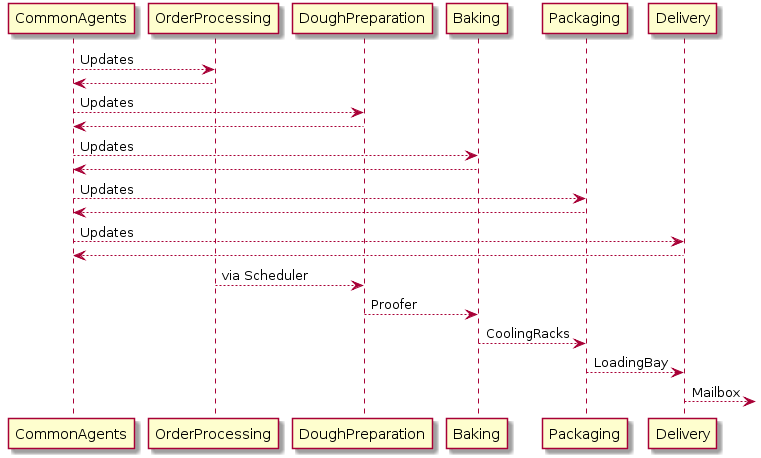
\includegraphics[scale=0.5]{../Architecture/Architecture_Stages.png}
	\caption{Architecture Overview}
	\label{architecture_overview}
\end{figure}

\pagebreak
\subsection{Communication between agents}
The agents belonging to each stage and the communication between them including the ACL messsage type are depicted in the figures mentioned in the description of the stages.

\begin{itemize}
	\item \textbf{Order Processing}: This stage deals with collecting orders from the customers, storing them until the day of delivery and scheduling the order for production on the day of delivery as shown in \ref{Architecture_OrderProcessing}.

\begin{figure}[h!]
	\centering
	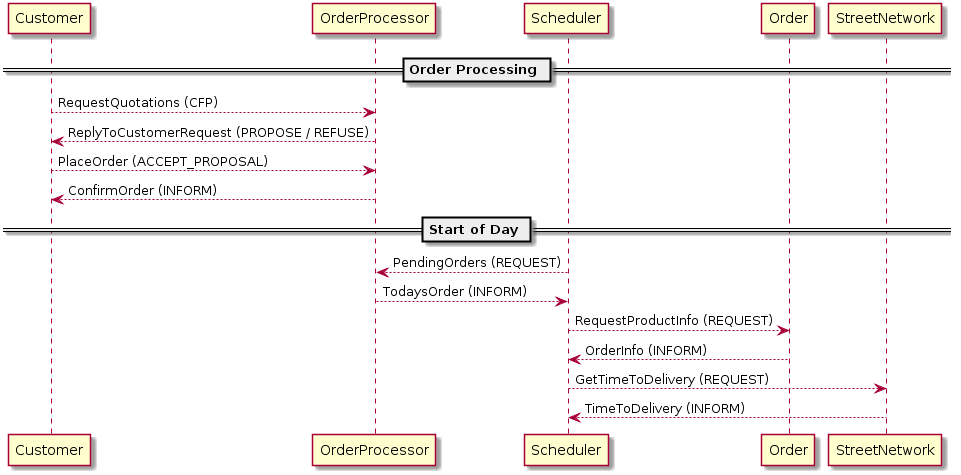
\includegraphics[scale=0.4]{../Architecture/Architecture_OrderProcessing.png}
	\caption{Order Processing}
	\label{Architecture_OrderProcessing}
\end{figure}	
	
	\item \textbf{Dough Preparation}: This stage deals with the Kneading of the dough, resting time and preparing the items for baking  as shown in \ref{Architecture_DoughPreparation}.
	
\begin{figure}[h!]
	\centering
	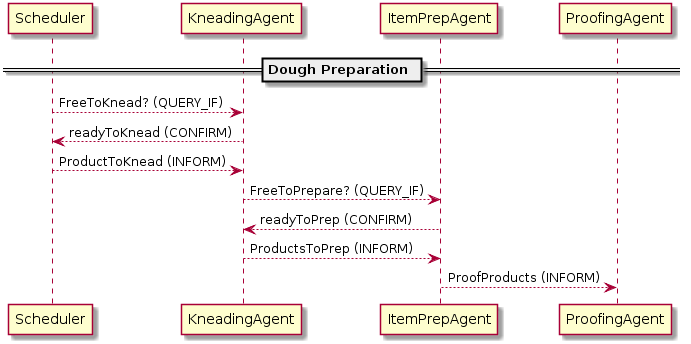
\includegraphics[scale=0.5]{../Architecture/Architecture_DoughPreparation.png}
	\caption{Dough Preparation}
	\label{Architecture_DoughPreparation}
\end{figure}	
	
	\item \textbf{Baking}: In this stage, the prepared items are filled on the trays, baked in the ovens, and cooled down  as shown in \ref{Architecture_Baking}..

\begin{figure}[h!]
	\centering
	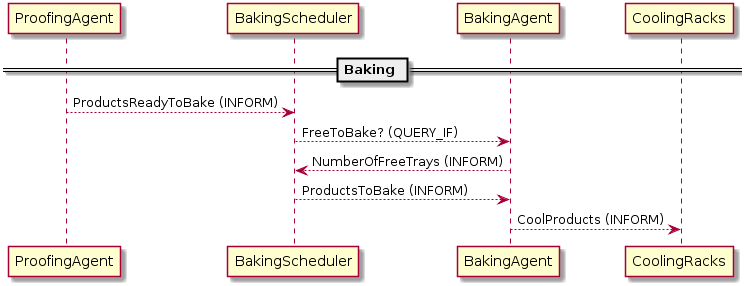
\includegraphics[scale=0.5]{../Architecture/Architecture_Baking.png}
	\caption{Baking}
	\label{Architecture_Baking}
\end{figure}	
	
	\item \textbf{Packing}: Here, the products are decorated and packaged into boxes for delivery  as shown in \ref{Architecture_Packaging}.
	
\begin{figure}[h!]
	\centering
	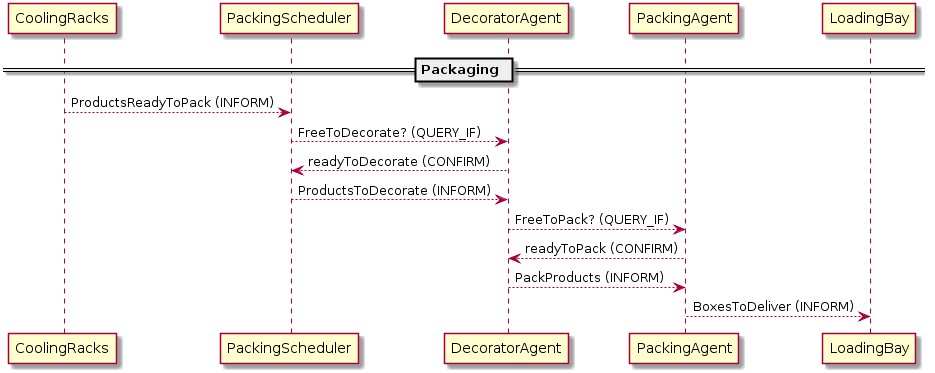
\includegraphics[scale=0.35]{../Architecture/Architecture_Packaging.png}
	\caption{Packing}
	\label{Architecture_Packaging}
\end{figure}	

	\item \textbf{Transportation}: This stage collects the prepared orders and uses Trucks to deliver the orders from the bakery to the customers  as shown in \ref{Architecture_Delivery}.
	
\begin{figure}[h!]
	\centering
	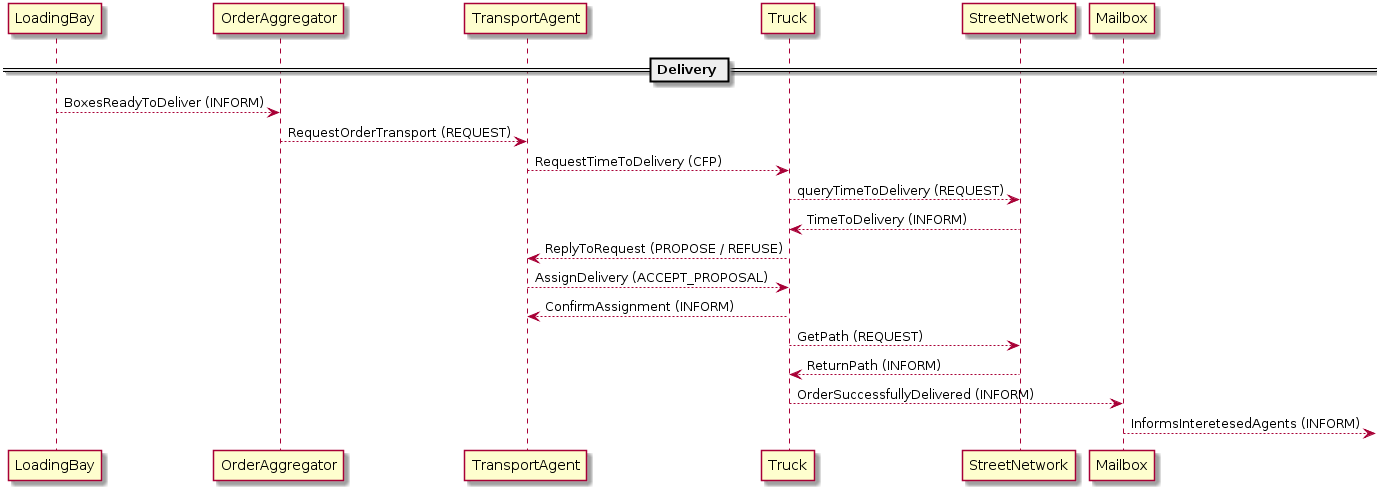
\includegraphics[scale=0.4]{../Architecture/Architecture_Delivery.png}
	\caption{Delivery}
	\label{Architecture_Delivery}
\end{figure}	
	
	\item \textbf{Common Agents}: This stage consists of agents that communicate with almost all the agents in the other stages. Candidate agents for this stage are the clock and the visualization agent.
\end{itemize}

\subsection{Agent Behaviors}
Every agent needs to have a set of behaviors to achieve its job. These are depicted in figure \ref{Agent_Behaviors}.
\begin{figure}[h!]
	\centering
	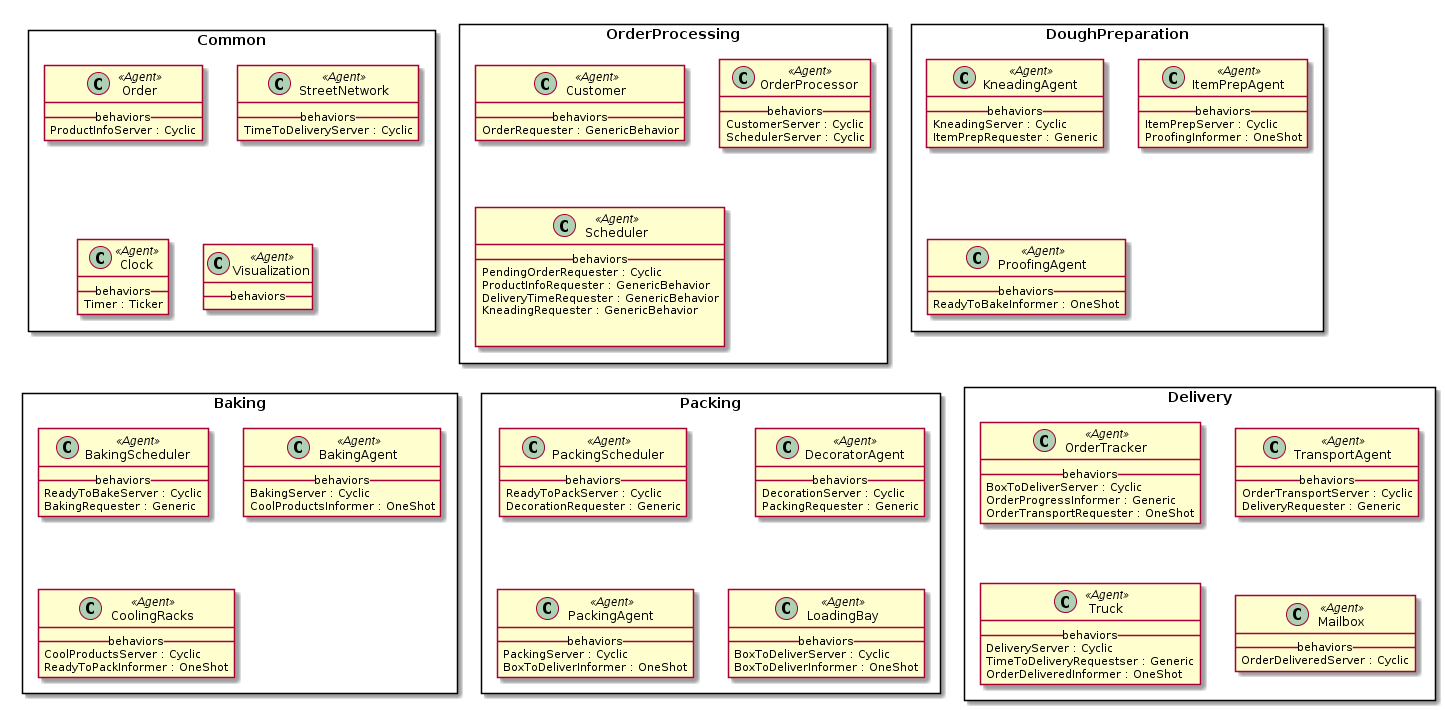
\includegraphics[scale=0.35]{../Architecture/AgentBehaviors.png}
	\caption{Agent Behaviors}
	\label{Agent_Behaviors}
\end{figure}	

\pagebreak
\section{Agent Definitions}

\begin{itemize}
	\item \textbf{Common}
	\begin{itemize}
	\item \textit{Component}: Clock
	\begin{itemize}
		\item \textit{Agent/Object} : Agent
		\item \textit{Static/Dynamic} : Static
		\item \textit{Description} : Maintains the system time and informs every other agent about time updates
	\end{itemize}
	\item \textit{Component}: Visualization Agent
	\begin{itemize}
		\item \textit{Agent/Object} : Agent
		\item \textit{Static/Dynamic} : Static
		\item \textit{Description} : Collects logging data from other agents and visualizes the overall system state
	\end{itemize}
	\item \textit{Component}: Order
	\begin{itemize}
		\item \textit{Agent/Object} : Agent
		\item \textit{Static/Dynamic} : Dynamic
		\item \textit{Description} : Maintains the list of items requested by the customer and updates it according to production status.
	\end{itemize}
	\item \textit{Component}: StreetNetwork
	\begin{itemize}
		\item \textit{Agent/Object} : Agent
		\item \textit{Static/Dynamic} : Static
		\item \textit{Description} : Handles service requests for time to deliver between two nodes in the map.
	\end{itemize}
	\end{itemize}

	\item \textbf{Order Processing}
	\begin{itemize}
	\item \textit{Component}:Customer
	\begin{itemize}
		\item \textit{Agent/Object} : Agent
		\item \textit{Static/Dynamic} : Dynamic
		\item \textit{Description} : Checks the quotations from every available bakery and places and order with one which has least quotation.
	\end{itemize}
	\item \textit{Component}: OrderProcessor
	\begin{itemize}
		\item \textit{Agent/Object} : Agent
		\item \textit{Static/Dynamic} : Static
		\item \textit{Description} : Provides quotations and collects order from customers. Also provides a list of orders pending for preparation to scheduler.
	\end{itemize}
	\item \textit{Component}: Scheduler
	\begin{itemize}
		\item \textit{Agent/Object} : Agent
		\item \textit{Static/Dynamic} : Static
		\item \textit{Description} : Schedules the orders for preparation based on their delivery time.
	\end{itemize}
	\item \textit{Component}: ProductInfo
	\begin{itemize}
		\item \textit{Agent/Object} : Object
		\item \textit{Static/Dynamic} : Static
		\item \textit{Description} : Contains all the details about a product (time to bake, etc.)
	\end{itemize}
	\end{itemize}

	\item \textbf{Dough Preparation}
	\begin{itemize}
	\item \textit{Component}: KneadingAgent
	\begin{itemize}
		\item \textit{Agent/Object} : Agent
		\item \textit{Static/Dynamic} : Static
		\item \textit{Description} : Handles the kneading and resting times for a product.
	\end{itemize}
	\item \textit{Component}: ItemPrepAgent
	\begin{itemize}
		\item \textit{Agent/Object} : Agent
		\item \textit{Static/Dynamic} : Static
		\item \textit{Description} : Prepares the items to be baked. Takes varying amount of time based on item to be prepared.
	\end{itemize}
	\item \textit{Component}: Proofer
	\begin{itemize}
		\item \textit{Agent/Object} : Agent
		\item \textit{Static/Dynamic} : Static
		\item \textit{Description} : Interface between the Dough preparation and Baking Stages.
	\end{itemize}
	\end{itemize}

	\item \textbf{Baking}
	\begin{itemize}
	\item \textit{Component}: BakingScheduler
	\begin{itemize}
		\item \textit{Agent/Object} : Agent
		\item \textit{Static/Dynamic} : Static
		\item \textit{Description} : Schedules the items to be backed based on the number of free ovens.
	\end{itemize}
	\item \textit{Component}: BakingAgent
	\begin{itemize}
		\item \textit{Agent/Object} : Agent
		\item \textit{Static/Dynamic} : Static
		\item \textit{Description} : Bakes the items in the oven after filling them in the tray.
	\end{itemize}
	\item \textit{Component}: CoolingRacks
	\begin{itemize}
		\item \textit{Agent/Object} : Agent
		\item \textit{Static/Dynamic} : Static
		\item \textit{Description} : Cools down the baked items and interfaces with the packing stage.
	\end{itemize}
	\end{itemize}

	\item \textbf{Packing}
	\begin{itemize}
	\item \textit{Component}: PackingScheduler
	\begin{itemize}
		\item \textit{Agent/Object} : Agent
		\item \textit{Static/Dynamic} : Static
		\item \textit{Description} : Schedules the cooled items for decoration.
	\end{itemize}
	\item \textit{Component}: DecoratorAgent
	\begin{itemize}
		\item \textit{Agent/Object} : Agent
		\item \textit{Static/Dynamic} : Static
		\item \textit{Description} : Decorates the baked items.
	\end{itemize}
	\item \textit{Component}: PackingAgent
	\begin{itemize}
		\item \textit{Agent/Object} : Agent
		\item \textit{Static/Dynamic} : Static
		\item \textit{Description} : Packs the decorated items into boxes.
	\end{itemize}
	\item \textit{Component}: LoadingBay
	\begin{itemize}
		\item \textit{Agent/Object} : Agent
		\item \textit{Static/Dynamic} : Static
		\item \textit{Description} : Interface between the packing and delivery stages.
	\end{itemize}
	\item \textit{Component}: Box
	\begin{itemize}
		\item \textit{Agent/Object} : Object
		\item \textit{Static/Dynamic} : Dynamic
		\item \textit{Description} : Used to store items to be delivered.
	\end{itemize}
	\end{itemize}

	\item \textbf{Delivery}
	\begin{itemize}
	\item \textit{Component}: OrderTracker
	\begin{itemize}
		\item \textit{Agent/Object} : Agent
		\item \textit{Static/Dynamic} : Static
		\item \textit{Description} : Interface between the packing and delivery stages.
	\end{itemize}
	\item \textit{Component}: TransportAgent
	\begin{itemize}
		\item \textit{Agent/Object} : Agent
		\item \textit{Static/Dynamic} : Static
		\item \textit{Description} : Requests the Truck agents to deliver the ready orders.
	\end{itemize}
	\item \textit{Component}: Truck
	\begin{itemize}
		\item \textit{Agent/Object} : Agent
		\item \textit{Static/Dynamic} : Static
		\item \textit{Description} : Collects the ready orders and delivers them to the customers.
	\end{itemize}
	\item \textit{Component}: Mailbox
	\begin{itemize}
		\item \textit{Agent/Object} : Agent
		\item \textit{Static/Dynamic} : Static
		\item \textit{Description} : Stores message sent by the trucks related to delivery status.
	\end{itemize}
	\end{itemize}
\end{itemize}


\newpage
\section{Aggregation of order data}

Since the proposed architectural skeleton requires the various stages in the production phase to be disjoint from each other, it was not possible to aggregate the orders efficiently. We instead propose that the orders be completed sequentially based on their time of delivery (early delivery orders will be picked first for preparation). In case two orders have the same delivery time and have an overlap between their desired products, we can merge the orders (produce identical items in both the orders together) to have some efficiency in the kneading and resting time of the dough. 

\end{document}\grid
